\section{Оборудование и инструментальные погрешности}
\subsection{Статический метод}

\begin{figure}[h!]
    \center{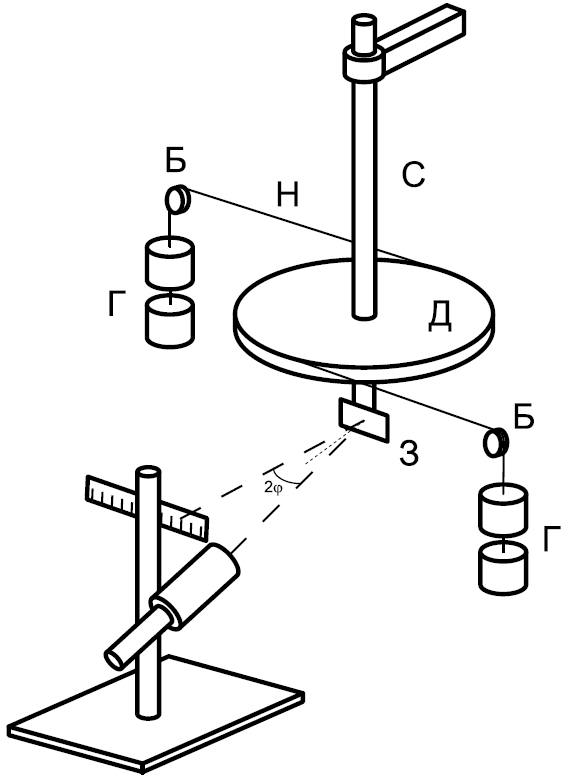
\includegraphics{img/static.png}}
\end{figure}

Схема установки приведена на рисунке. Верхний конец стержня С
жёстко закреплён на стойке, а нижний соединён с диском Д. момент
создают две нити, навитые на него и перекинутые через блоки Б. К
их концам подвешиваются одинаковые грузы Г. Диск сабжён Зеркальцем
З. Для определения угла закручивания стержня надо направить зрительную
трубку на зеркальце и добиться того, чтобы в неё было чётко видно
отражение шкалы, укреплённой на том же штативе. Измерение смещения
шкалы позволяет определить угол закручивания стержня.

\subsection{Метод крутильных колебаний}
\begin{figure}[h!]
    \center{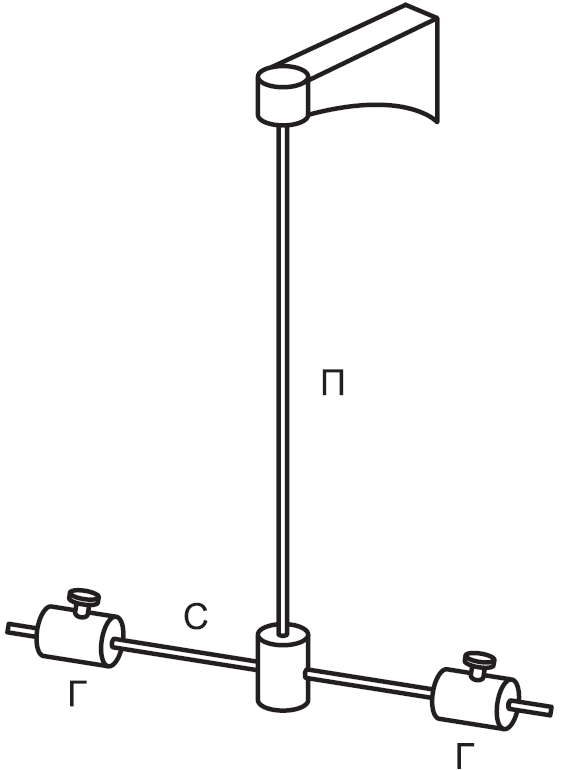
\includegraphics{img/spin.png}}
\end{figure}

Схема установки приведена на рисунке. Она состоит длинной висящей
проволоки П, к нижнему концу которой прикреплён горизонтальный
стержень С с двумя симметрично расположенными грузами Г. Их
положение можно фиксировать. Верхний конец проволоки зажат и может
поворачиваться вокруг оси. Так можно возбуждать крутильные колебания.

Вращение стержня происходит под действием упругого момента. Это
вращение описывается уравнением:
\[I\frac{d^2\varphi}{dt^2}=-M\]
$I$~--- момент иннерции стержня с грузами относительно оси вращения,
$\varphi$~--- угол поворота от положения равновесия, $M$~--- момент сил.
\[\omega^2=\frac{f}{I}\]
тогда
\[\frac{d^2\varphi}{dt^2}+\omega^2\varphi=0\]
\[\varphi=\varphi_0\sin\left(\omega t + \theta\right)\]
Амплитуда $\varphi_0$ и фаза $\theta$ опреедляются начальными условиями.

Период колебаний
\[T=\frac{2\pi}{\omega}=2\pi\sqrt{\frac{I}{f}}\]

Эти уравнения получены для незатухающий колебаний, поэтому для Их
применения в работе необходимо убедиться, что колебания затухают слабо
(амплитуда уменьшается менее, чем в 2 раза за 10 колебаний). Также
надо убедиться, что период колебаний не зависит от начальной амплитуды.
Начальную амплитуду необходимо уменьшать пока зависимость от амплитуды
не исчезнет.

Момент иннерции системы
\[I=I_0+2m\left(r+\frac{b}{2}\right)^2\]
$I$~--- момент иннерции системы без грузов, $m$~--- масса одного груза,
$r$~--- расстояние от ближнего торца груза до проволоки, $b$~--- длина груза.
\[T^2=\frac{\left(2\pi\right)^2}{f}I_0 + \frac{\left(2\pi\right)^2}{f}2m\left(r+\frac{b}{2}\right)^2\]
График этой зависимости в координатах $T^2\left(\left(r+b/2\right)^2\right)$ будет линейным
с наклоном $k=\frac{8\pi^2m}{f}$, откуда $f=\frac{8\pi^2m}{k}$.
